\documentclass[aspectratio=169,12pt]{beamer}
\usetheme{Madrid}
\usecolortheme{dolphin}
\usefonttheme{professionalfonts}
\setbeamertemplate{navigation symbols}{}
\setbeamertemplate{footline}{}

\usepackage[T1]{fontenc}
\usepackage[utf8]{inputenc}
\usepackage{graphicx}
\usepackage{amsmath,amssymb}
\usepackage{hyperref}
\usepackage{siunitx}
\usepackage{physics}
\usepackage{braket}

\graphicspath{{../../figures/}}

\title[Module B3]{Module B3: Qiskit -- exécution sur QPU}
\author{JAMOTTE Maxime, SCHOONEN Cédric}
\institute{Digital Learning Hub}
\date{}

\begin{document}

\begin{frame}
  \titlepage
\end{frame}

\begin{frame}{Objectifs du module B3}
  \begin{itemize}
    \item Différentes backends (vrais QPUs et simulateurs)\\~\\
    \item Transpilation\\~\\
    \item Primitives\\~\\
    \item Démo avec une paire de Bell
  \end{itemize}
\end{frame}

% ============================================================
\section{Backends}
% ============================================================

\begin{frame}{Différentes backends}
  \begin{itemize}[<+->]
    \setlength{\itemsep}{0.8em}
    \item \textbf{Simulateurs}: exécution sur ordinateur classique (ex: \texttt{AerSimulator}).\\~\\
    \item \textbf{QPUs réels}: processeurs quantiques accessibles via IBM Quantum (ex: \texttt{ibm\_brisbane}).\\~\\
    \item Les simulateurs sont utiles pour le développement et le débogage.\\~\\
    \item Les QPUs réels introduisent du bruit (erreurs de portes, décohérence).
  \end{itemize}
\end{frame}

% ============================================================
\section{Transpilation}
% ============================================================

\begin{frame}{Transpilation : Six Étapes}
  \begin{columns}[T]
    \begin{column}{0.58\textwidth}
      \small
      \vspace{-0.7em}
      \begin{enumerate}
        \setlength{\itemsep}{0.3em}
        \item \textbf{Init}: Réduction des opérations multi-qubits en portes à 1 et 2 qubits (Optionnel)
        \item \textbf{Layout}: Assignation des qubits physiques
        \item \textbf{Routing}: Insertion de portes SWAP pour déplacer les états quantiques entre qubit (NP-difficile, algorithme aléatoire)
        \item \textbf{Translation}: Conversion de toutes les portes vers le jeu d'instructions natif (ISA)
        \item \textbf{Optimization}: Remplacement ou élimination de portes logiques où c'est possible
        \item \textbf{Scheduling}: Insertion de délais (Optionnel)
      \end{enumerate}
    \end{column}
    \begin{column}{0.4\textwidth}
      \centering
      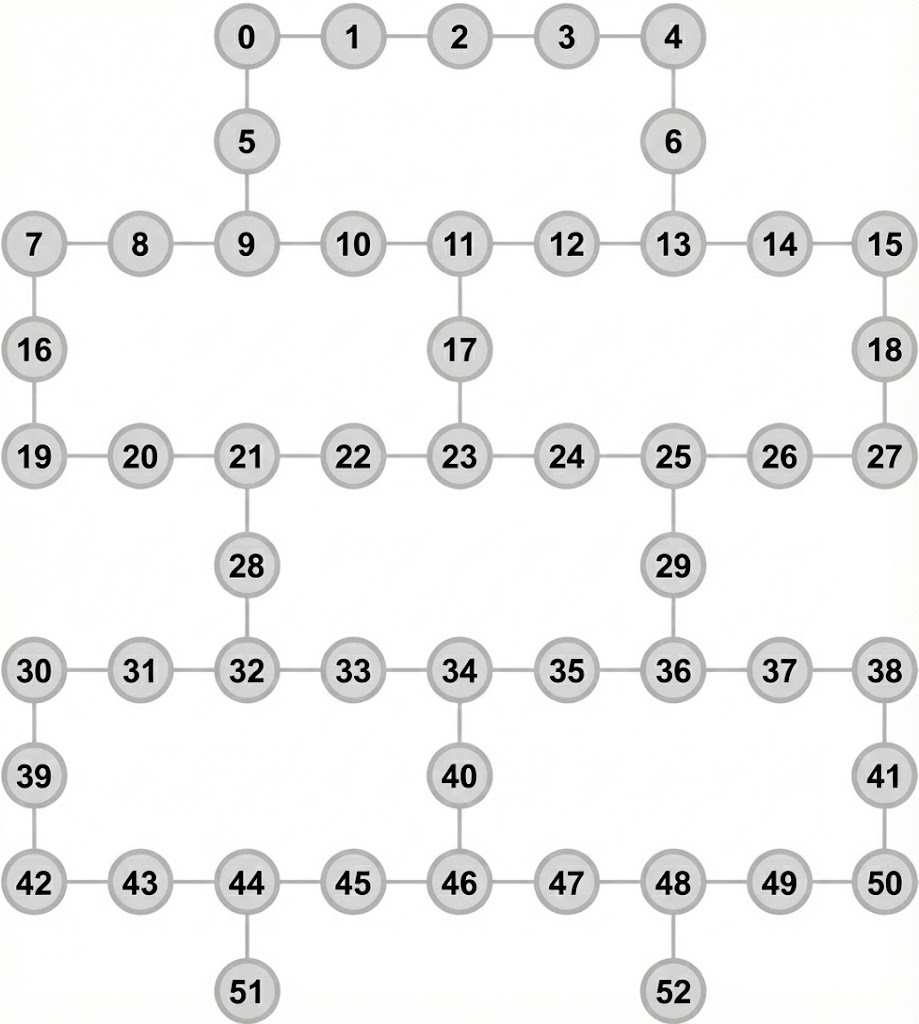
\includegraphics[width=\textwidth]{qubits_layout.jpg}
    \end{column}
  \end{columns}
\end{frame}

\begin{frame}{Transpilation: Niveaux d'Optimisation}
  \small
  \begin{description}
    \setlength{\itemsep}{1.5em}
    \item[\textbf{Niveau 1}:] Combination matricielle des portes à un qubit,\\ élimination des portes CNOT redondantes
    
    \item[\textbf{Niveau 2}:] Analyse de commutation pour éliminer davantage de redondances
    
    \item[\textbf{Niveau 3}:] Optimisation des sous-blocs à deux qubits identifiés dans le circuit\\ (reconstruit une matrice unitaire équivalente)
  \end{description}
\end{frame}

% ============================================================
\section{Primitives}
% ============================================================

\begin{frame}{Primitives Qiskit}
  \begin{itemize}[<+->]
    \setlength{\itemsep}{0.8em}
    \item Les \textbf{primitives} sont l'interface standard pour exécuter des circuits.\\~\\
    \item \texttt{Sampler}: exécute le circuit et retourne un échantillon de résultats de mesure.\\~\\
    \item \texttt{Estimator}: estime la valeur moyenne d'une observable.\\~\\
    \item Disponibles pour simulateurs et QPUs réels.
  \end{itemize}
\end{frame}

% ============================================================
\section{Démo avec une paire de Bell}
% ============================================================

\begin{frame}{Démo: paire de Bell sur QPU (voir JN)}
  \begin{itemize}[<+->]
    \item Construire le circuit de la paire de Bell.\\~\\
    \item Transpiler pour le backend cible.\\~\\
    \item Exécuter avec le \texttt{Sampler} (1000 shots).\\~\\
    \item Analyser les résultats: on attend $\approx 50\%$ de $\ket{00}$ et $\approx 50\%$ de $\ket{11}$.\\~\\
    \item Sur un vrai QPU, on observera aussi du bruit (quelques $\ket{01}$ et $\ket{10}$).
  \end{itemize}
\end{frame}

\begin{frame}{Fin du module B3}
  \centering
  \vfill
  Vers les applications!
  \vfill
\end{frame}

\end{document}
